% ============================================================================
% TEMPLATE PARA TRABAJOS PRÁCTICOS INDIVIDUALES (TPI)
% Asignatura: Ampliación de Bases de Datos
% Curso 2026/2027 - Universidad Loyola Andalucía
%
% TPI 2: Big Data y Bases de Datos a Gran Escala (Spark SQL + PostgreSQL)
% Estudiante: Fernando Martín González
% Profesor: Dr. Anier Soria Lorente
% Repositorio: https://github.com/fernandomartin04/spark-mercadona-ventas
% ============================================================================

\documentclass[a4paper,12pt]{article}

% ---------------------------------------------------------------------------
% Codificación, idioma y tipografía
% ---------------------------------------------------------------------------
\usepackage[utf8]{inputenc}
\usepackage[T1]{fontenc}
\usepackage[spanish,es-nodecimaldot]{babel}
\usepackage{lmodern}
\usepackage{microtype}
\usepackage{eurosym}

% ---------------------------------------------------------------------------
% Página y espaciado
% ---------------------------------------------------------------------------
\usepackage[a4paper,top=2.3cm,bottom=2.3cm,left=2.5cm,right=2.5cm]{geometry}
\usepackage{setspace}
\setstretch{1.12}
\setlength{\parindent}{0pt}
\setlength{\parskip}{0.5em}

% ---------------------------------------------------------------------------
% Colores e identidad visual (Universidad Loyola)
% ---------------------------------------------------------------------------
\usepackage{xcolor}
\definecolor{LoyolaBlue}{HTML}{082B66}
\definecolor{LoyolaCyan}{HTML}{5CC8DF}
\definecolor{SoftBlue}{HTML}{EEF5FA}
\definecolor{SoftGray}{HTML}{F5F6F7}
\definecolor{TextGray}{HTML}{374151}

% ---------------------------------------------------------------------------
% Imágenes, tablas y listas
% ---------------------------------------------------------------------------
\usepackage{graphicx}
\usepackage{booktabs}
\usepackage{array}
\usepackage{enumitem}
\usepackage{float}
\usepackage{caption}

% ---------------------------------------------------------------------------
% Código fuente
% ---------------------------------------------------------------------------
\usepackage{listings}
\lstdefinestyle{codigo}{
  basicstyle=\ttfamily\footnotesize,
  backgroundcolor=\color{SoftGray},
  frame=single,
  rulecolor=\color{LoyolaBlue!35},
  numbers=left,
  numberstyle=\tiny\color{TextGray},
  numbersep=6pt,
  breaklines=true,
  showstringspaces=false,
  tabsize=2,
  captionpos=b,
  keywordstyle=\color{LoyolaBlue}\bfseries,
  commentstyle=\color{green!45!black},
  stringstyle=\color{orange!60!black},
  literate={á}{{\'a}}1 {é}{{\'e}}1 {í}{{\'i}}1 {ó}{{\'o}}1 {ú}{{\'u}}1 {ñ}{{\~n}}1 {º}{{\textordmasculine}}1
}
\lstset{style=codigo}

% ---------------------------------------------------------------------------
% Matemáticas y enlaces
% ---------------------------------------------------------------------------
\usepackage{amsmath,amssymb}
\usepackage{url}
\usepackage[hidelinks]{hyperref}
\hypersetup{
  colorlinks=true,
  linkcolor=LoyolaBlue,
  urlcolor=LoyolaBlue,
  citecolor=LoyolaBlue,
  pdftitle={TPI 2 - Big Data con Spark SQL e Integracion Empresarial},
  pdfauthor={Fernando Martín González}
}

% ---------------------------------------------------------------------------
% Cabecera y pie de página
% ---------------------------------------------------------------------------
\usepackage{fancyhdr}
\usepackage{lastpage}
\pagestyle{fancy}
\fancyhf{}
\fancyhead[L]{\small\textcolor{LoyolaBlue}{Ampliación de Bases de Datos}}
\fancyhead[R]{\small\textcolor{TextGray}{TPI 2 - Spark SQL}}
\fancyfoot[L]{\small Universidad Loyola Andalucía}
\fancyfoot[R]{\small Página \thepage\ de \pageref{LastPage}}
\renewcommand{\headrulewidth}{0.6pt}
\renewcommand{\headrule}{\hbox to\headwidth{\color{LoyolaCyan}\leaders\hrule height \headrulewidth\hfill}}
\renewcommand{\footrulewidth}{0pt}

% ---------------------------------------------------------------------------
% Estilo de secciones
% ---------------------------------------------------------------------------
\usepackage{titlesec}
\titleformat{\section}{\large\bfseries\color{LoyolaBlue}}{\thesection.}{0.5em}{}
\titleformat{\subsection}{\normalsize\bfseries\color{LoyolaBlue}}{\thesubsection.}{0.5em}{}

% ---------------------------------------------------------------------------
% DATOS DEL TRABAJO
% ---------------------------------------------------------------------------
\newcommand{\TPINumero}{TPI 2}
\newcommand{\TPITitulo}{Análisis de Ventas por Tramos Horarios y Productos Más Vendidos en Mercadona mediante Spark SQL y PostgreSQL}
\newcommand{\Estudiante}{Fernando Martín González}
\newcommand{\FechaEntrega}{Octubre de 2026}
\newcommand{\Profesor}{Dr. Anier Soria Lorente}
\newcommand{\RepoURL}{https://github.com/fernandomartin04/spark-mercadona-ventas}

\begin{document}

% ============================================================================
% PORTADA
% ============================================================================
\begin{titlepage}
  \thispagestyle{empty}
  \begin{center}
    
\includegraphics[width=0.65\textwidth]{logo_uloyola.png}

    \vspace{1.0cm}
    {\Large\bfseries\color{LoyolaBlue} Ampliación de Bases de Datos\par}
    \vspace{0.2cm}
    {\large Grado en Ingeniería del Software\par}
    {\large Curso académico 2026/2027\par}

    \vspace{1.2cm}
    \colorbox{SoftBlue}{%
      \parbox{0.88\textwidth}{%
        \centering
        \vspace{0.4cm}
        {\LARGE\bfseries\color{LoyolaBlue}\TPINumero\par}
        \vspace{0.3cm}
        {\large\bfseries\TPITitulo\par}
        \vspace{0.4cm}
      }%
    }

    \vfill
    \begin{tabular}{>{\bfseries}p{4.2cm} p{9.0cm}}
      Estudiante: & \Estudiante \\
      Profesor: & \Profesor \\
      Fecha de entrega: & \FechaEntrega \\
      Repositorio GitHub: & \footnotesize\url{\RepoURL} \\
    \end{tabular}

    \vfill
    {\small\color{TextGray} Universidad Loyola Andalucía}
  \end{center}
\end{titlepage}

% ============================================================================
% ÍNDICE
% ============================================================================
\tableofcontents
\newpage

% ============================================================================
% 1. PROBLEMA REAL Y CONTEXTO
% ============================================================================
\section{Problema real y contexto}

La idea de este trabajo parte de cómo funciona un supermercado como Mercadona en su día a día. Cada vez que una cajera cobra a un cliente, cada producto que pasa por el lector genera una línea de venta con la hora exacta, el código del producto, las unidades y el precio en euros. En una sola tienda hay varias cajas funcionando a la vez y, si sumamos varios supermercados de una ciudad o del país, en una sola jornada se acumulan decenas de miles o millones de líneas de ticket en ficheros CSV enormes.

Con ese volumen de datos en bruto, un encargado o el departamento de operaciones de Mercadona necesita saber dos cosas muy sencillas pero fundamentales para gestionar la tienda:
\begin{enumerate}[leftmargin=1.0cm]
    \item \textbf{Cuál es la venta media en euros (\euro{}) por cada hora y por cada 30 minutos:} Por ejemplo, si de 13:00 a 14:00 se venden 20.000~\euro{} y de 14:00 a 15:00 se venden 30.000~\euro{}, saber qué se factura en cada tramo y cuál es la media del día para ver qué horas están por encima o por debajo de lo normal.
    \item \textbf{Cuál es el producto más vendido en cada tramo de 30 minutos o de 1 hora:} Saber qué artículo se está agotando más rápido en cada momento del día para reponer las estanterías a tiempo.
\end{enumerate}

Para llevarlo a la práctica de forma realista sin que el archivo ocupe demasiado espacio en el ordenador ni en GitHub, hemos generado un dataset de \textbf{50.000 líneas de venta} (\texttt{ventas\_mercadona.csv}) repartidas a lo largo de las 12 horas de apertura de un día (de 09:00 a 21:00) en cinco tiendas de Sevilla.

Todo el código, los datos y la configuración de Docker están disponibles en el repositorio público de GitHub: \url{\RepoURL}.

% ============================================================================
% 2. NECESIDAD RELACIONADA CON LOS DATOS Y OBJETIVOS
% ============================================================================
\section{Necesidad relacionada con los datos y objetivos}

\subsection{Necesidad identificada}
Si abrimos un fichero CSV con decenas de miles o millones de ventas en un Excel tradicional, el programa va lento o directamente se bloquea. Y si metiéramos todas esas filas en bruto en la base de datos de las cajas para hacer sumas y medias cada pocos minutos, saturaríamos el sistema transaccional mientras las cajeras están cobrando.

Por tanto, necesitamos separar el problema en dos pasos: usar un motor de Big Data (\textbf{Spark SQL}) que lea el CSV masivo en memoria y haga todos los cálculos pesados, y luego guardar únicamente las tablas con el resultado ya resumido en una base de datos relacional (\textbf{PostgreSQL}) para poder consultarlo desde una página web sencilla.

\subsection{Objetivo general}
Procesar un archivo masivo de 50.000 ventas de Mercadona mediante Apache Spark SQL para obtener la venta media y el producto más vendido en tramos de 1 hora y de 30 minutos, integrando los resultados en PostgreSQL y mostrándolos en un panel web sencillo.

\subsection{Objetivos específicos}
\begin{itemize}[leftmargin=1.0cm]
  \item Desplegar un entorno con Docker Compose que conecte un contenedor de Apache Spark 3.5 y otro de PostgreSQL 16.
  \item Generar un fichero CSV con 50.000 ventas realistas de productos de Mercadona con fecha y hora (\texttt{timestamp}), unidades e importe.
  \item Implementar consultas claras en \textbf{Spark SQL} (Apartado 5.4) para agrupar ventas por tramos de 1 hora y 30 minutos, calcular la recaudación media y obtener el producto número 1 de cada franja.
  \item Volcar las tablas finales de resultados a PostgreSQL mediante el conector \textbf{JDBC} (Apartado 5.5) y crear un visor HTML sencillo para consultar los datos.
\end{itemize}

% ============================================================================
% 3. CONCEPTOS Y TECNOLOGÍAS APLICADAS
% ============================================================================
\section{Conceptos y tecnologías aplicadas}

\subsection{Procesamiento con Spark SQL (Apartado 5.4)}
Spark SQL es el módulo de Apache Spark que permite trabajar con datos estructurados (como nuestro CSV de 50.000 filas) ejecutando consultas SQL directamente en memoria RAM. En nuestro proyecto cumple tres funciones:
\begin{itemize}[leftmargin=1.0cm]
    \item \textbf{Lectura y vistas temporales:} Lee el archivo \texttt{ventas\_mercadona.csv} detectando automáticamente los tipos de datos (\texttt{inferSchema=True}) y lo registra como una tabla temporal en memoria (\texttt{createOrReplaceTempView}).
    \item \textbf{Clasificación por tramos horarios:} Con funciones SQL sencillas (\texttt{DATE\_FORMAT}, \texttt{MINUTE} y \texttt{CASE WHEN}), asigna cada venta a su bloque de 1 hora (ej. \texttt{12:00}) y de 30 minutos (ej. \texttt{12:00} o \texttt{12:30}).
    \item \textbf{Funciones de agregación y de ventana:} Utiliza \texttt{SUM()}, \texttt{COUNT()} y \texttt{AVG() OVER} para calcular el dinero recaudado y la venta media por tramo, y \texttt{ROW\_NUMBER() OVER} para ordenar los productos de mayor a menor venta en cada franja y quedarse con el primero.
\end{itemize}

\subsection{Integración con sistemas de información empresarial (Apartado 5.5)}
En una empresa real, los encargados de tienda no abren una terminal de Spark para ver qué se está vendiendo. El papel de la integración empresarial consiste en conectar Spark con la base de datos de negocio (\textbf{PostgreSQL}) usando el driver oficial \textbf{JDBC} (\texttt{postgresql-42.7.4.jar}).

Así, Spark lee las 50.000 filas en bruto, hace las cuentas y escribe en PostgreSQL solo \textbf{dos tablas ligeras de 36 filas cada una} (\texttt{resumen\_ventas\_tramo} y \texttt{producto\_mas\_vendido\_tramo}). De esta forma, la página web de consulta lee los resultados al instante sin tener que procesar las 50.000 ventas cada vez que alguien entra.

\subsection{Contenerización con Docker Compose}
Hemos configurado dos servicios dentro de una misma red de Docker (\texttt{mercadona\_net}): \texttt{mercadona\_spark} (con la imagen oficial \texttt{apache/spark:3.5.3-python3}) y \texttt{mercadona\_postgres} (con \texttt{postgres:16-alpine}).

% ============================================================================
% 4. DESARROLLO DEL TRABAJO
% ============================================================================
\section{Desarrollo del trabajo}

\subsection{Estructura de los datos de entrada (CSV)}
El script \texttt{scripts/01\_generar\_datos.py} crea el fichero \texttt{data/ventas\_mercadona.csv} con 50.000 ventas repartidas entre las 09:00 y las 20:59. Cada fila representa un paso por caja con las siguientes columnas:
\begin{itemize}[leftmargin=1.0cm]
    \item \texttt{id\_venta}: Identificador único de la venta (del 1 al 50.000).
    \item \texttt{fecha\_hora}: Timestamp exacto (ej. \texttt{2026-10-24 12:14:32}).
    \item \texttt{id\_tienda}: Supermercado de Sevilla donde se realiza la compra.
    \item \texttt{id\_producto} y \texttt{nombre\_producto}: Artículo del catálogo de Mercadona (leche, cerveza, guacamole, pizza, huevos, etc.).
    \item \texttt{cantidad}, \texttt{precio\_unitario} e \texttt{importe\_total}: Unidades compradas y total en euros (\euro{}).
\end{itemize}

\subsection{Consultas en Spark SQL}
En el script \texttt{scripts/02\_procesar\_spark\_sql.py} cargamos el CSV y ejecutamos tres consultas SQL muy sencillas y fáciles de seguir. En primer lugar, clasificamos cada venta en su tramo de 1 hora y de 30 minutos:

\begin{lstlisting}[language=SQL,caption={Clasificación de cada venta en tramos de 1 hora y de 30 minutos}]
SELECT
    id_venta, fecha_hora, id_tienda, id_producto,
    nombre_producto, cantidad, importe_total,
    DATE_FORMAT(fecha_hora, 'HH:00') AS tramo_1h,
    -- Si el minuto es menor que 30 va a la primera media hora (:00), y si no a (:30)
    CASE
        WHEN MINUTE(fecha_hora) < 30 THEN DATE_FORMAT(fecha_hora, 'HH:00')
        ELSE DATE_FORMAT(fecha_hora, 'HH:30')
    END AS tramo_30m
FROM ventas_brutas
\end{lstlisting}

En segundo lugar, agrupamos por tramo horario para sumar la recaudación en euros y calculamos la media global del día con \texttt{AVG()}:

\begin{lstlisting}[language=SQL,caption={Cálculo de la recaudación por tramo y la venta media en euros}]
-- 1. Sumamos las ventas y el dinero recaudado en cada tramo
SELECT '1_HORA' AS tipo_ventana, tramo_1h AS franja_horaria,
       COUNT(*) AS numero_ventas, ROUND(SUM(importe_total), 2) AS recaudacion_euros
FROM ventas_con_tramos
GROUP BY tramo_1h
UNION ALL
SELECT '30_MIN' AS tipo_ventana, tramo_30m AS franja_horaria,
       COUNT(*) AS numero_ventas, ROUND(SUM(importe_total), 2) AS recaudacion_euros
FROM ventas_con_tramos
GROUP BY tramo_30m;

-- 2. Calculamos la media entre todos los tramos de 1 hora y de 30 minutos
SELECT tipo_ventana, franja_horaria, numero_ventas, recaudacion_euros,
       ROUND(AVG(recaudacion_euros) OVER (PARTITION BY tipo_ventana), 2) AS media_global_euros
FROM tramos_agrupados
ORDER BY tipo_ventana, franja_horaria;
\end{lstlisting}

Por último, para saber cuál es el producto más vendido en cada tramo, sumamos las unidades vendidas de cada artículo, las ordenamos de mayor a menor con \texttt{ROW\_NUMBER()} y filtramos el puesto número 1:

\begin{lstlisting}[language=SQL,caption={Obtención del producto más vendido en cada tramo}]
SELECT tipo_ventana, franja_horaria, id_producto,
       nombre_producto, unidades_totales, euros_producto
FROM (
    SELECT *,
           ROW_NUMBER() OVER (
               PARTITION BY tipo_ventana, franja_horaria
               ORDER BY unidades_totales DESC -- El que tenga mas unidades sale el 1
           ) AS posicion
    FROM ventas_por_producto
)
WHERE posicion = 1
ORDER BY tipo_ventana, franja_horaria;
\end{lstlisting}

\subsection{Exportación JDBC a PostgreSQL y Panel Web}
Una vez calculados los dos DataFrames en Spark, se envían directamente a la base de datos \texttt{mercadona\_bi} de PostgreSQL mediante \texttt{write.jdbc()}. Finalmente, el script \texttt{scripts/03\_generar\_panel\_web.py} lee las dos tablas desde PostgreSQL y genera el archivo \texttt{panel\_mercadona.html}.

% ============================================================================
% 5. RESULTADOS OBTENIDOS
% ============================================================================
\section{Resultados obtenidos}

En la Figura~\ref{fig:spark} se muestra la ejecución del script de PySpark en la terminal, donde lee las 50.000 filas del CSV y muestra por pantalla las tablas calculadas antes de guardarlas en PostgreSQL.

\begin{figure}[H]
  \centering
  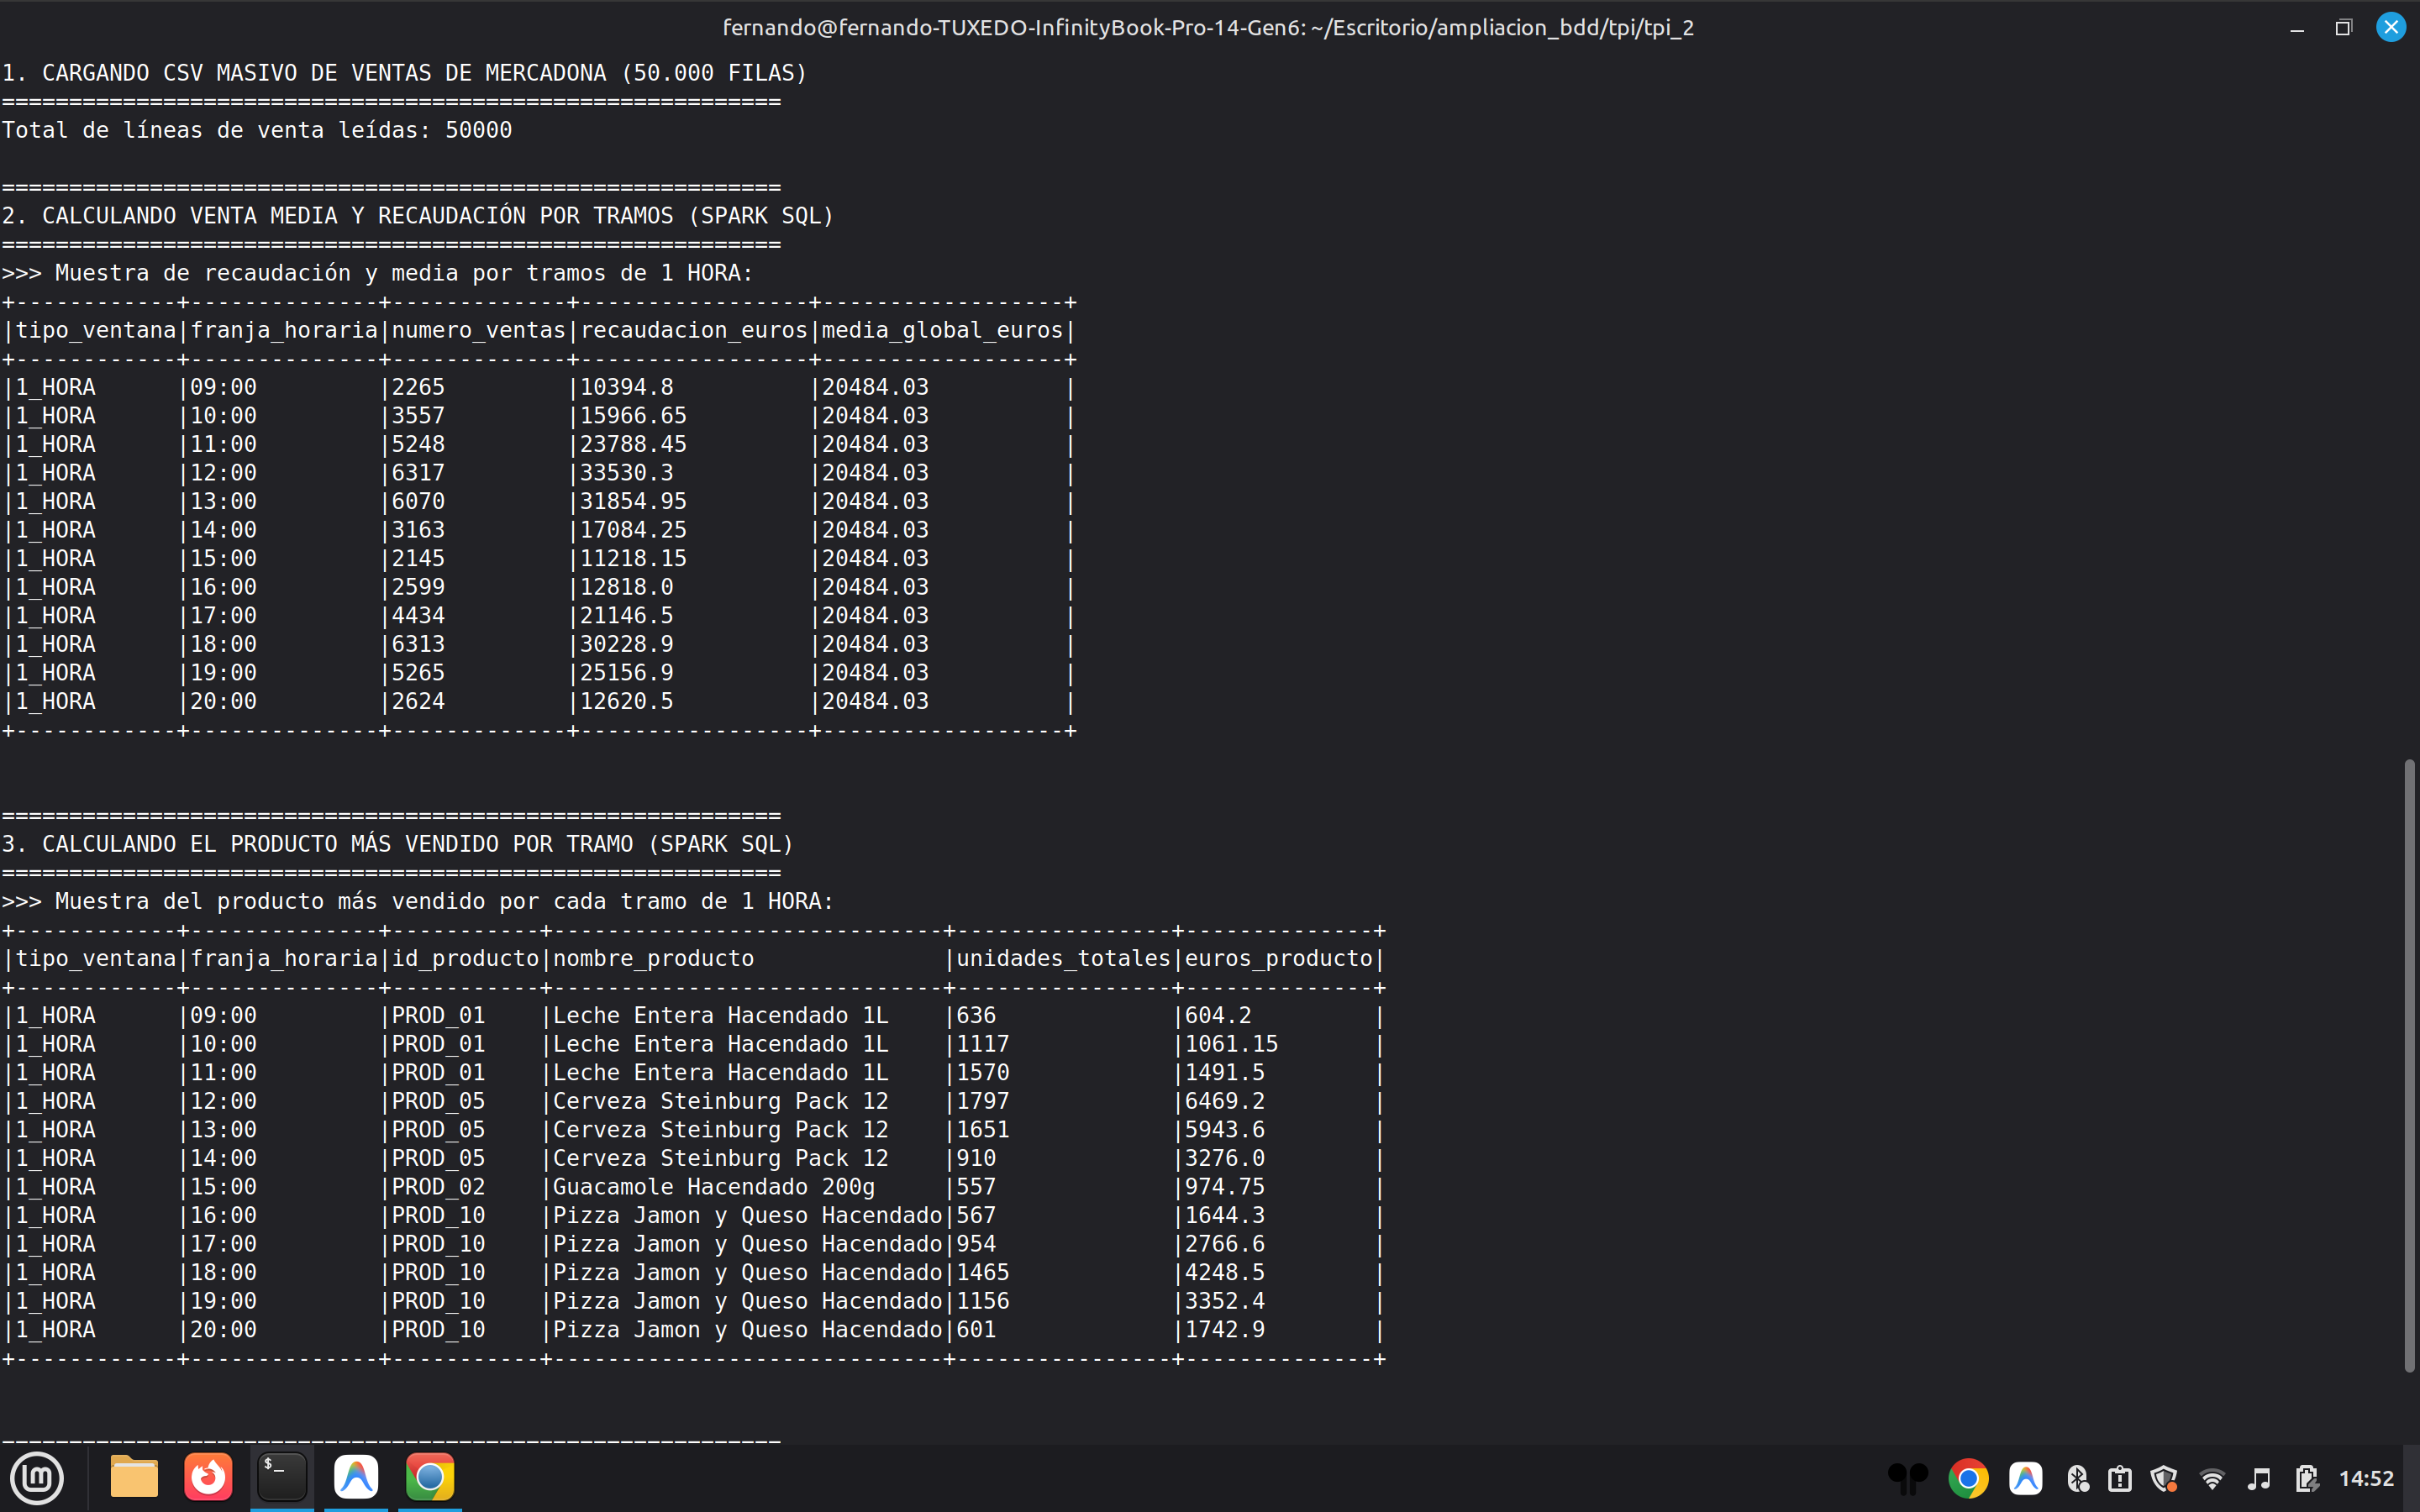
\includegraphics[width=0.92\textwidth]{imgs/captura_spark.png}
  \caption{Ejecución de Spark SQL procesando las 50.000 ventas y calculando las medias y el top de productos.}
  \label{fig:spark}
\end{figure}

En la Figura~\ref{fig:postgres} se comprueba que ambos contenedores Docker están activos y que los datos ya están guardados dentro de PostgreSQL consultando las tablas \texttt{resumen\_ventas\_tramo} y \texttt{producto\_mas\_vendido\_tramo}.

\begin{figure}[H]
  \centering
  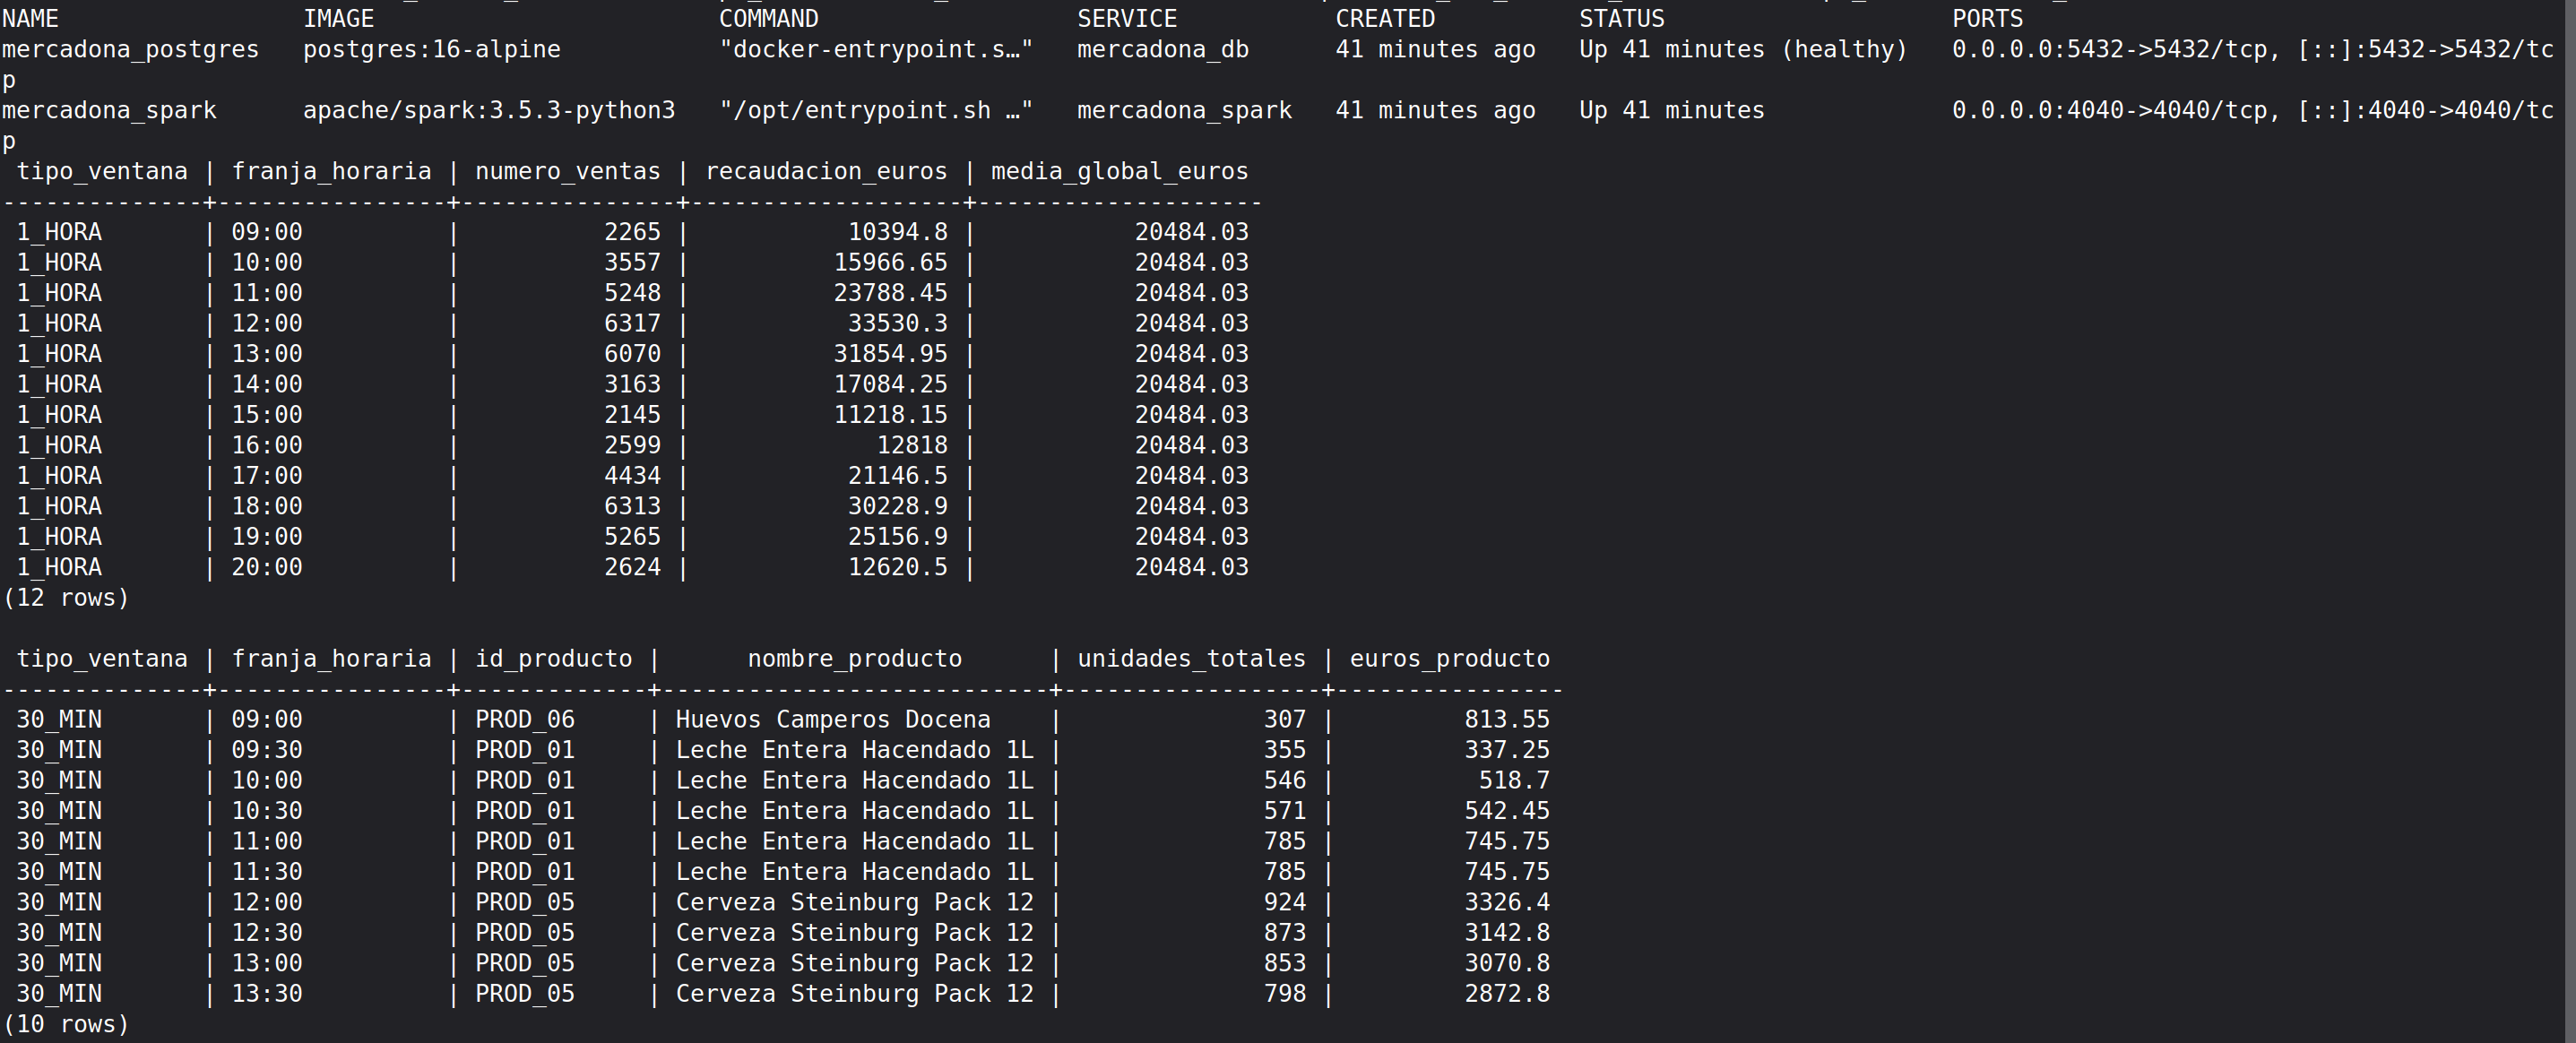
\includegraphics[width=0.92\textwidth]{imgs/captura_postgres.png}
  \caption{Verificación de los contenedores Docker y consulta directa de las tablas en PostgreSQL.}
  \label{fig:postgres}
\end{figure}

En la Tabla~\ref{tab:resultados} se resumen los resultados obtenidos por tramos de 1 hora (con una \textbf{venta media de 20.484,03~\euro{} por hora}, y de \textbf{10.242,01~\euro{} cada 30 minutos}):

\begin{table}[H]
  \centering
  \small
  \caption{Resumen de recaudación, media por hora y producto más vendido en el día.}
  \label{tab:resultados}
  \begin{tabular}{cccc l c}
    \toprule
    \textbf{Franja} & \textbf{Ventas} & \textbf{Recaudación (\euro{})} & \textbf{Media 1h (\euro{})} & \textbf{Producto Más Vendido} & \textbf{Uds.} \\
    \midrule
    09:00 & 2.265 & 10.394,80 & 20.484,03 & Leche Entera Hacendado 1L & 636 \\
    10:00 & 3.557 & 15.966,65 & 20.484,03 & Leche Entera Hacendado 1L & 1.117 \\
    11:00 & 5.248 & 23.788,45 & 20.484,03 & Leche Entera Hacendado 1L & 1.570 \\
    \textbf{12:00} & \textbf{6.317} & \textbf{33.530,30} & \textbf{20.484,03} & \textbf{Cerveza Steinburg Pack 12} & \textbf{1.797} \\
    13:00 & 6.070 & 31.854,95 & 20.484,03 & Cerveza Steinburg Pack 12 & 1.651 \\
    14:00 & 3.163 & 17.084,25 & 20.484,03 & Cerveza Steinburg Pack 12 & 910 \\
    15:00 & 2.145 & 11.218,15 & 20.484,03 & Guacamole Hacendado 200g & 557 \\
    16:00 & 2.599 & 12.818,00 & 20.484,03 & Pizza Jamón y Queso Hacendado & 567 \\
    17:00 & 4.434 & 21.146,50 & 20.484,03 & Pizza Jamón y Queso Hacendado & 954 \\
    18:00 & 6.313 & 30.228,90 & 20.484,03 & Pizza Jamón y Queso Hacendado & 1.465 \\
    19:00 & 5.265 & 25.156,90 & 20.484,03 & Pizza Jamón y Queso Hacendado & 1.156 \\
    20:00 & 2.624 & 12.620,50 & 20.484,03 & Pizza Jamón y Queso Hacendado & 601 \\
    \bottomrule
  \end{tabular}
\end{table}

Por último, en la Figura~\ref{fig:panel} se muestra la página web desarrollada (\texttt{panel\_mercadona.html}), donde el usuario puede cambiar en un clic entre tramos de \textbf{1 Hora} y de \textbf{30 Minutos}, elegir cualquier franja horaria y ver al instante la venta media y el producto más vendido.

\begin{figure}[H]
  \centering
  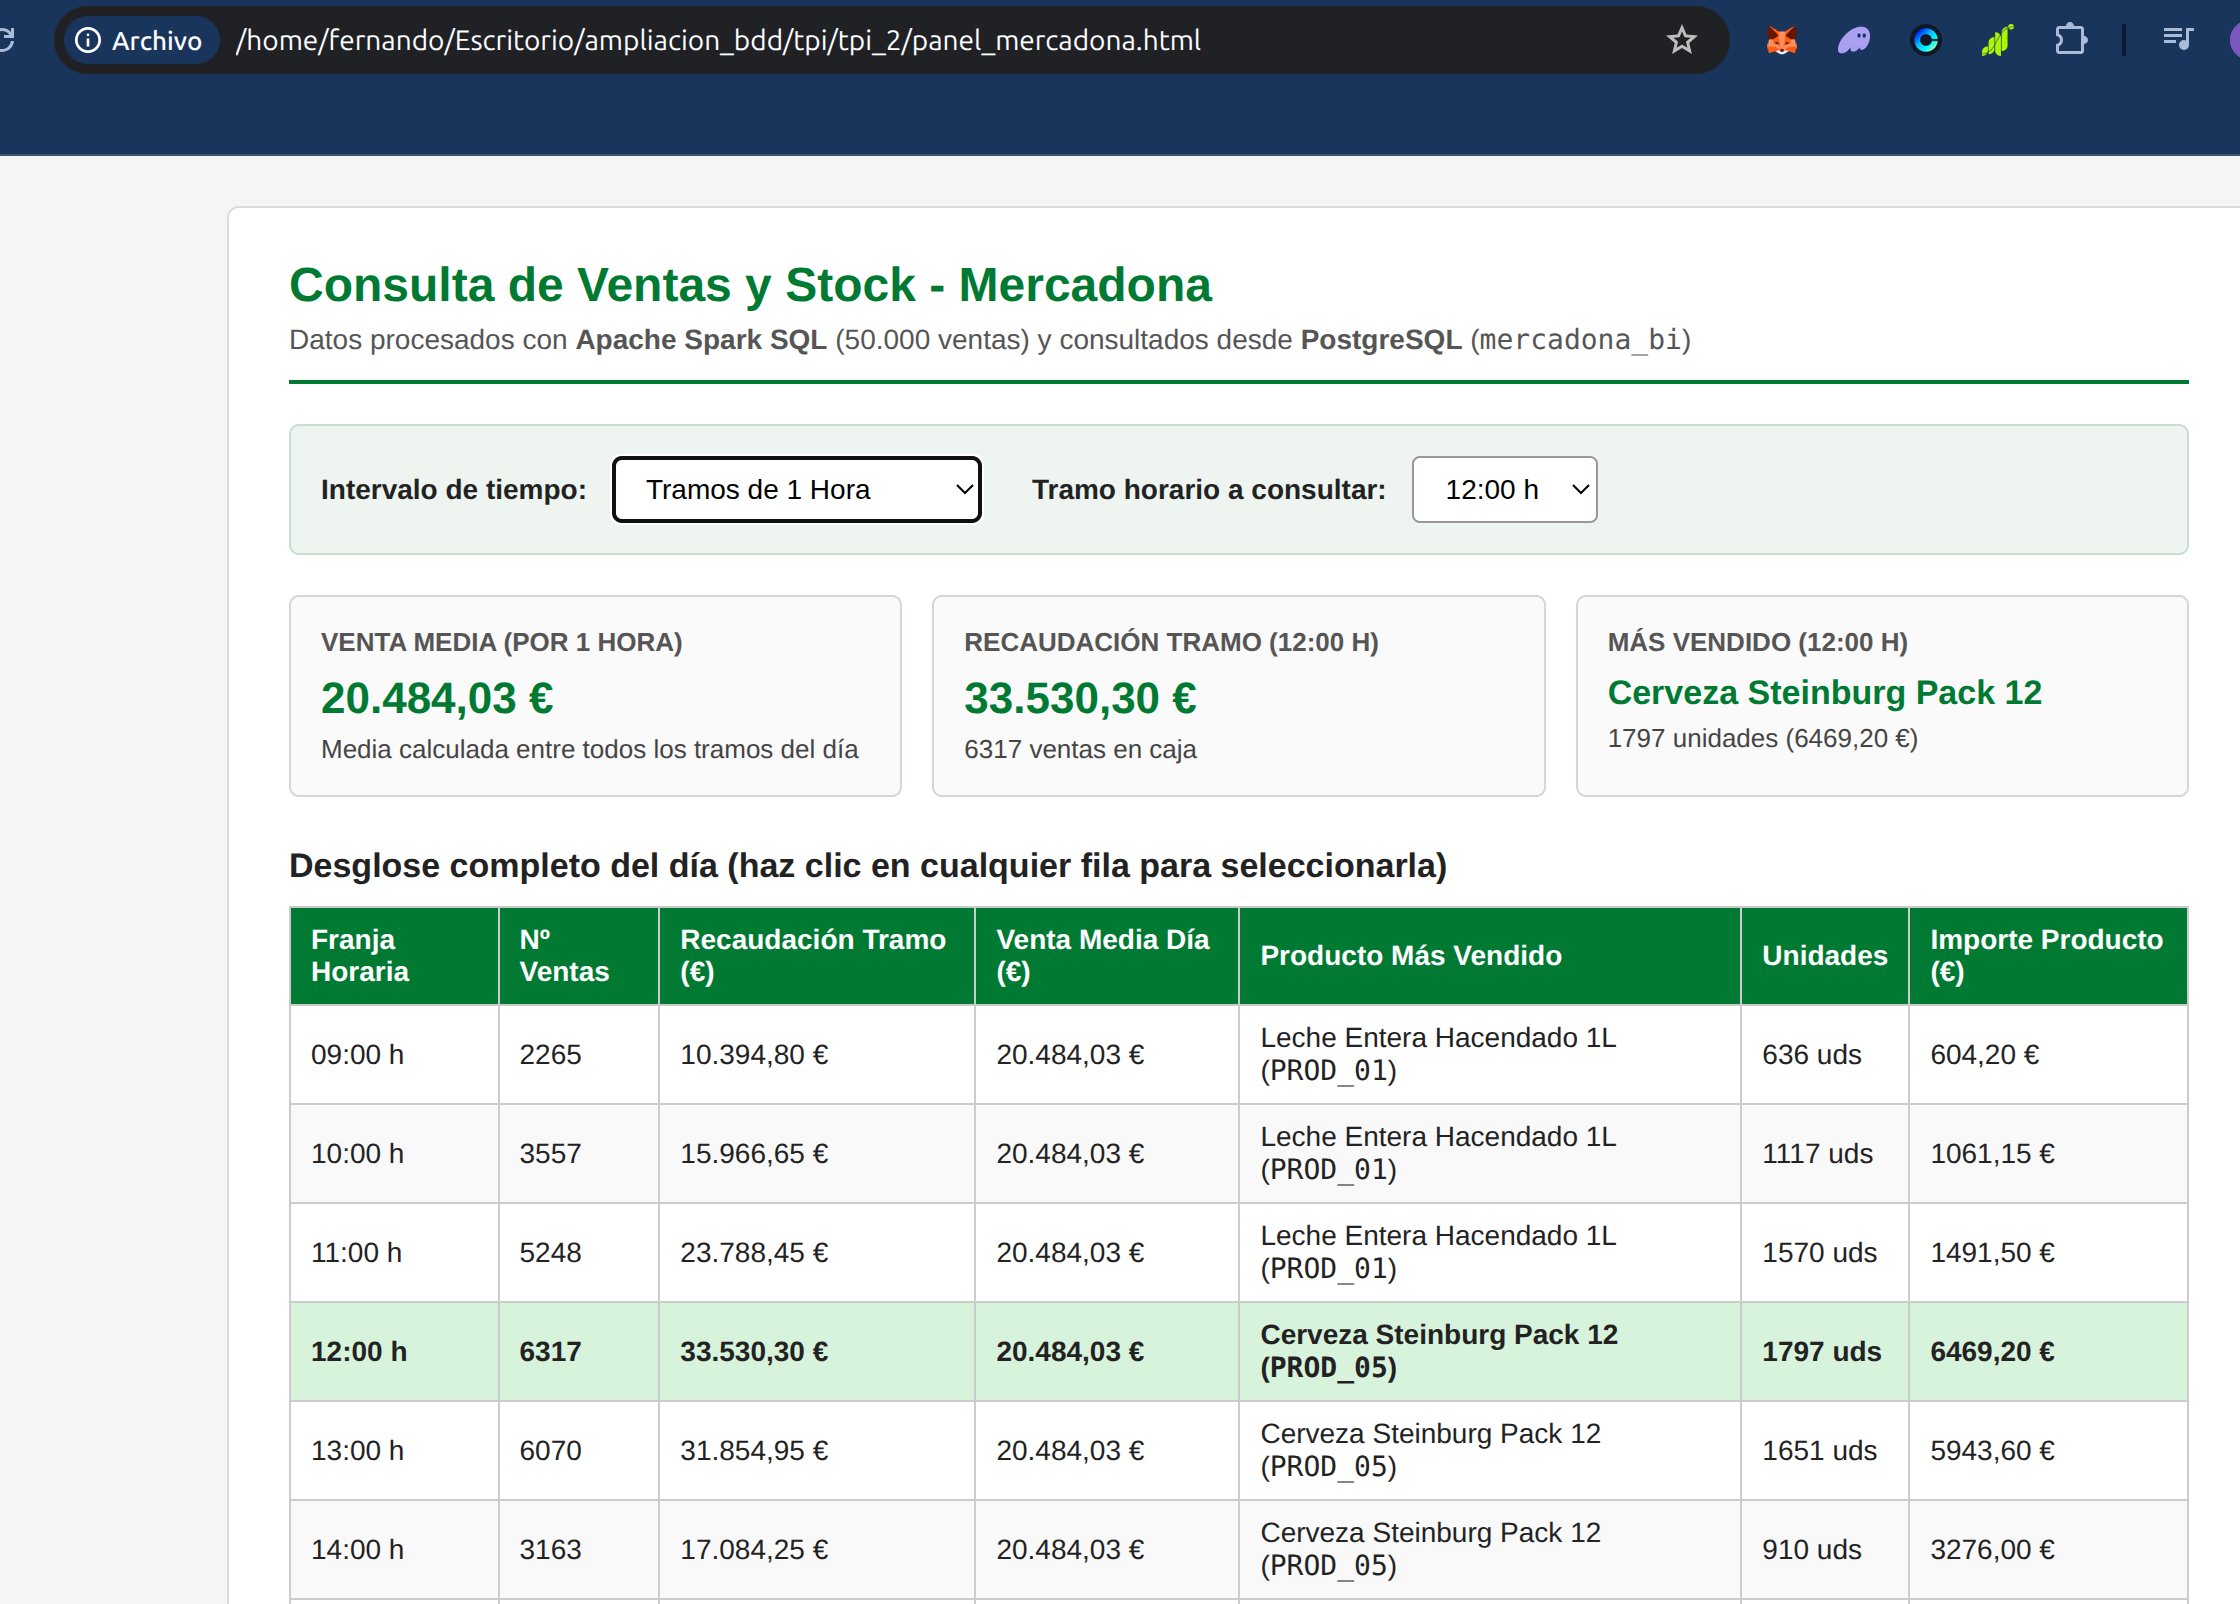
\includegraphics[width=0.90\textwidth]{imgs/captura_panel.png}
  \caption{Interfaz web sencilla conectada a los resultados almacenados en PostgreSQL.}
  \label{fig:panel}
\end{figure}

% ============================================================================
% 6. ANÁLISIS E INTERPRETACIÓN
% ============================================================================
\section{Análisis e interpretación de los resultados}

A partir de los resultados obtenidos se pueden sacar tres conclusiones muy claras:
\begin{enumerate}[leftmargin=1.0cm]
    \item \textbf{Utilidad de la venta media frente a las horas punta:} La facturación total del día es de 245.808,35~\euro{}. Al dividirla entre las 12 horas de apertura obtenemos la media de \textbf{20.484,03~\euro{}/hora} (y \textbf{10.242,01~\euro{}} en medias de 30 minutos). Esto permite ver de un vistazo qué horas tiran hacia arriba del supermercado (como las 12:00 con 33.530,30~\euro{} o las 18:00 con 30.228,90~\euro{}) y cuáles son horas valle (como las 09:00 o las 15:00, que rondan los 10.000--11.000~\euro{}).
    \item \textbf{Cambio del producto más vendido según el tramo:} Al mirar los datos por horas y cada 30 minutos se ve claramente cómo cambia lo que compra la gente: a primera hora (09:00 a 09:30) ganan los \textit{Huevos Camperos} y la \textit{Leche Hacendado}; al mediodía (12:00 a 14:30) se dispara el pack de \textit{Cerveza Steinburg} y a las 15:00 el \textit{Guacamole}; mientras que por la tarde-noche domina la \textit{Pizza Jamón y Queso}.
    \item \textbf{Reducción de datos gracias a Spark SQL:} Hemos pasado de un archivo de 50.000 líneas de venta a solo 36 filas en PostgreSQL (12 filas para los tramos de 1 hora y 24 filas para los tramos de 30 minutos). Así la base de datos de la empresa se mantiene limpia y rapidísima.
\end{enumerate}

% ============================================================================
% 7. DECISIONES TOMADAS Y JUSTIFICACIÓN
% ============================================================================
\section{Decisiones tomadas y justificación}

\begin{itemize}[leftmargin=1.0cm]
  \item \textbf{Volumen de 50.000 filas en CSV:} Elegimos 50.000 ventas (~4,4 MB) porque es un tamaño suficiente para justificar el procesamiento automatizado con Spark SQL frente a una hoja de cálculo, pero a la vez ligero para ejecutarlo en segundos en local y poder subirlo entero a GitHub sin problemas.
  \item \textbf{Consultas SQL sencillas y legibles:} En lugar de usar expresiones complejas o código enrevesado, hemos usado funciones SQL estándar (\texttt{CASE WHEN}, \texttt{GROUP BY}, \texttt{SUM}, \texttt{AVG} y \texttt{ROW\_NUMBER}) que se entienden a la primera lectura.
  \item \textbf{Separar el análisis (Spark) del almacenamiento (PostgreSQL):} En lugar de meter las 50.000 ventas en PostgreSQL, Spark hace el cálculo bruto en memoria y solo envía por JDBC las dos tablas finales ya resumidas.
  \item \textbf{Interfaz HTML directa y sin recargar:} Se ha creado un visor web limpio que permite alternar entre 30 minutos y 1 hora sin depender de servidores complejos.
\end{itemize}

% ============================================================================
% 8. CONCLUSIONES Y APRENDIZAJE
% ============================================================================
\section{Conclusiones y aprendizaje}

Con este trabajo hemos visto de forma práctica para qué sirve combinar Spark SQL con una base de datos relacional como PostgreSQL. Hemos comprobado que Spark SQL permite tratar ficheros grandes de decenas de miles de filas como si fueran tablas normales de SQL, agrupando por tramos de tiempo y sacando rankings en un par de segundos.

Además, la integración mediante JDBC demuestra cómo trabajan las empresas en la realidad: el motor de Big Data se encarga de masticar los datos brutos y deja en PostgreSQL únicamente las tablas resumen limpias para que las aplicaciones o páginas web de la empresa funcionen de forma inmediata.

% ============================================================================
% 9. DECLARACIÓN DE USO DE INTELIGENCIA ARTIFICENCIA
% ============================================================================
\section{Declaración de uso de inteligencia artificial}

\textbf{Marque una opción y complete la información correspondiente:}

\begin{itemize}[label=$\square$,leftmargin=1.0cm]
  \item No he utilizado herramientas de inteligencia artificial en la realización de este trabajo.
  \item[\rlap{$\square$}{\raisebox{2pt}{\large\hspace{1pt}\textbf{X}}}] \textbf{Sí he utilizado herramientas de inteligencia artificial} como apoyo en este trabajo.
\end{itemize}

\textbf{Herramienta(s) utilizada(s):} \\
Google Gemini / Antigravity.

\textbf{Uso concreto realizado:} \\
Se utilizó como apoyo para configurar el entorno de Docker Compose con Apache Spark y PostgreSQL, consultar la conexión mediante el driver JDBC en PySpark, estructurar el visor HTML y asistir en la maquetación del documento en LaTeX siguiendo la plantilla de la asignatura.

\textbf{Revisión y validación personal:} \\
La idea original del caso de Mercadona, el diseño de las tablas y la lógica de tramos de 30 minutos y 1 hora han sido propuestos y dirigidos personalmente. Todos los scripts de generación de datos, las consultas de Spark SQL y la integración con PostgreSQL han sido ejecutados y comprobados en mi propia terminal local para asegurar que comprendo cada paso de cara a la defensa oral.

% ============================================================================
% 10. REFERENCIAS
% ============================================================================
\section{Referencias}

\begin{thebibliography}{9}

\bibitem{repo_github}
Fernando Martín González,
\textit{Análisis de Ventas en Mercadona mediante Spark SQL y PostgreSQL (Docker)},
Repositorio en GitHub, 2026.
\url{https://github.com/fernandomartin04/spark-mercadona-ventas}

\bibitem{spark_sql_doc}
Apache Software Foundation,
\textit{Spark SQL, DataFrames and Datasets Guide (Spark 3.5.3)},
2024.
\url{https://spark.apache.org/docs/3.5.3/sql-programming-guide.html}

\bibitem{postgres_jdbc_doc}
PostgreSQL Global Development Group,
\textit{PostgreSQL JDBC Driver Documentation},
2024.
\url{https://jdbc.postgresql.org/documentation/}

\bibitem{postgres_doc}
PostgreSQL Global Development Group,
\textit{PostgreSQL 16 Documentation},
2024.
\url{https://www.postgresql.org/docs/16/}

\end{thebibliography}

\end{document}
